\documentclass[12pt,aspectratio=169]{beamer}

\usetheme{CSCS}

\graphicspath{{./figs/}}

% define footer text
\newcommand{\footlinetext}{Directive Based GPU Programming course 2018}

% Select the image for the title page
\newcommand{\picturetitle}{cscs_images/cscs_entrance_painting.pdf}

\lstdefinestyle{shstyle}{
  basicstyle=\scriptsize\ttfamily,
  keywordstyle=\color{blue},
  stringstyle=\color{magenta},
  commentstyle=\itshape\color{cscsred},
  language=bash,
}

\newcommand\shinline[2][]{\lstinline[style=shstyle,basicstyle=\ttfamily,#1]!#2!}

% Please use the predifined colors:
% cscsred, cscsgrey, cscsgreen, cscsblue, cscsbrown, cscspurple, cscsyellow,
% cscsblack, cscswhite

\author{\emph{Vasileios Karakasis, CSCS}}
\title{Introduction to the Piz Daint environment}
\subtitle{Directive Based GPU Programming}
\date{May 14--15, 2018}


\begin{document}

% TITLE SLIDE
\cscstitle

\begin{frame}{Overview}
  \begin{itemize}
  \item Accessing CSCS
  \item Compiling my code
  \item Running my code
  \item Editing my code
  \item Transferring files from/to CSCS
  \item Repository of the course
  \end{itemize}
\end{frame}

\begin{frame}{Piz Daint}{Computing nodes}
  Piz Daint is a hybrid cluster of Cray XC40/XC50 nodes
  \begin{itemize}
  \item Hybrid nodes (XC50)
    \begin{itemize}
    \item 5320 total
    \item Intel\textregistered\ Xeon\textregistered\ E5-2690 v3 @ 2.60GHz (12 cores, 64GB RAM, Haswell)
    \item NVIDIA\textregistered\ Tesla\textregistered\ P100 16GB (Pascal)
    \end{itemize}
  \item Multicore nodes
    \begin{itemize}
    \item 1813 nodes
    \item Two Intel\textregistered\ Xeon\textregistered E5-2695 v4 @ 2.10GHz (2 x 18 cores, 64/128 GB RAM, Broadwell)
    \end{itemize}
  \item Login nodes
    \begin{itemize}
    \item 5 total
    \item Intel\textregistered\ Xeon\textregistered CPU E5-2650 v3 @ 2.30GHz (10 cores, 256 GB RAM, Haswell)
    \end{itemize}
  \item Aries routing and communications ASIC, and Dragonfly network topology
  \end{itemize}
\end{frame}

\begin{frame}{Piz Daint}{Filesystems}
  \begin{itemize}
  \item \texttt{/scratch}: High performance Lustre filesystem accessible from the computing nodes
    \begin{itemize}
    \item Environment variable \shinline{$SCRATCH} points to it
    \item Total capacity: 6.2\,PB
    \item Must be used for heavy I/O
    \end{itemize}
  \item \texttt{/users}: GPFS filesystem for the users' homes
  \item \texttt{/project}, \texttt{/store}: Long-term storage for computational projects
  \end{itemize}
  \vfill
  More on \url{https://user.cscs.ch/storage/file_systems/}
\end{frame}

\begin{frame}[fragile]{Accessing Piz Daint}
  \begin{itemize}
  \item Accessible through SSH
  \item Piz Daint is not directly accessible from the outside world:
    \begin{itemize}
    \item \texttt{ela} $\rightarrow$ \texttt{daint10x} $\rightarrow$ \texttt{nidxxxxx}
    \end{itemize}
  \end{itemize}

  Two-steps process:
  \begin{enumerate}
  \item Login to the frontend, forwarding X11 (will be needed the second day)
  \item Move to the login nodes of Piz Daint
  \end{enumerate}

  \vfill
  \begin{lstlisting}[style=shstyle]
# Login to the frontend first
ssh -Y courseXX@ela.cscs.ch
ssh -Y daint
  \end{lstlisting}
\end{frame}

\begin{frame}[fragile]{Programming Environments}
  Cray Linux Programming Environment
  \begin{itemize}
  \item 4 compilers available: \texttt{CCE}, \texttt{GNU}, \texttt{INTEL}, \texttt{PGI}
  \item 4 predefined Programming Environments:
    \begin{itemize}
    \item PrgEnv-\texttt{cray} (default), \texttt{PrgEnv-gnu}, \texttt{PrgEnv-intel}, \texttt{PrgEnv-pgi}
    \item \shinline{echo $PE_ENV} to get the current PrgEnv
    \end{itemize}
  \item 3 wrappers available: \texttt{ftn} (Fortran), \texttt{cc} (C), \texttt{CC} (C++)
    \begin{itemize}
    \item Required for compiling MPI programs
    \item They set appropriate optimisation flags for the target architecture (CPU or GPU)
    \item They provide a sort of portability across the programming environments
    \end{itemize}
  \end{itemize}
\end{frame}


\begin{frame}{Managing programming environments}
  Daint uses \emph{Environment Modules} (TMod) for managing the programming
  environments and the software packages:
  \vspace\baselineskip
  \begin{itemize}
  \item Dynamic modification of a user's environment via \emph{modulefiles}.
  \item All programming environments and software on Daint is available through modules.
  \item The compiler wrappers will detect the loaded programming environment
    and automatically set the correct flags and libraries.
  \end{itemize}
\end{frame}


\begin{frame}{Managing programming environments}{Listing modules}
  \begin{itemize}
  \item[--] \shinline{module list}
  \end{itemize}
  {
    \centering
    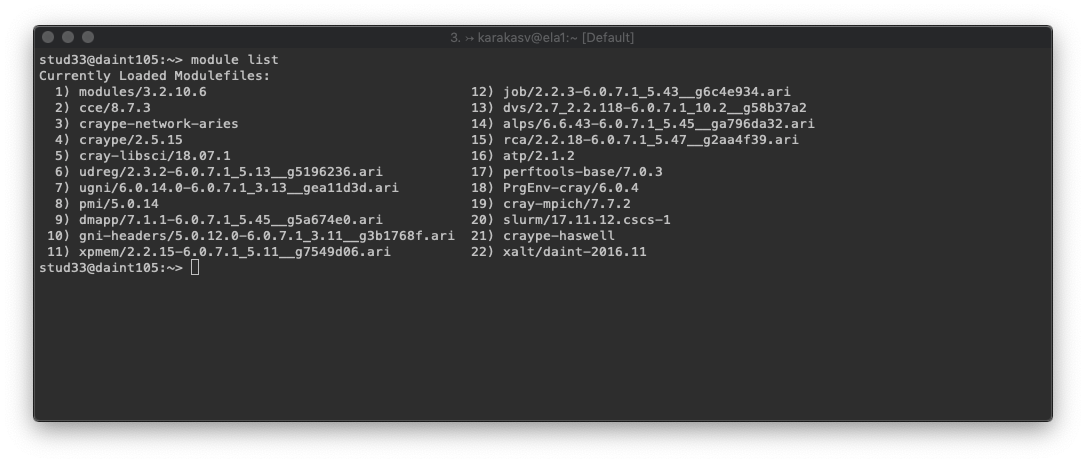
\includegraphics[width=\textwidth]{module_list.png}
  }
\end{frame}

\begin{frame}{Managing programming environments}{Switching programming environments}
  \begin{itemize}
  \item[--] Switch to the PGI programming environment
  \item[--] \shinline{module switch}
  \end{itemize}
  {
    \centering
    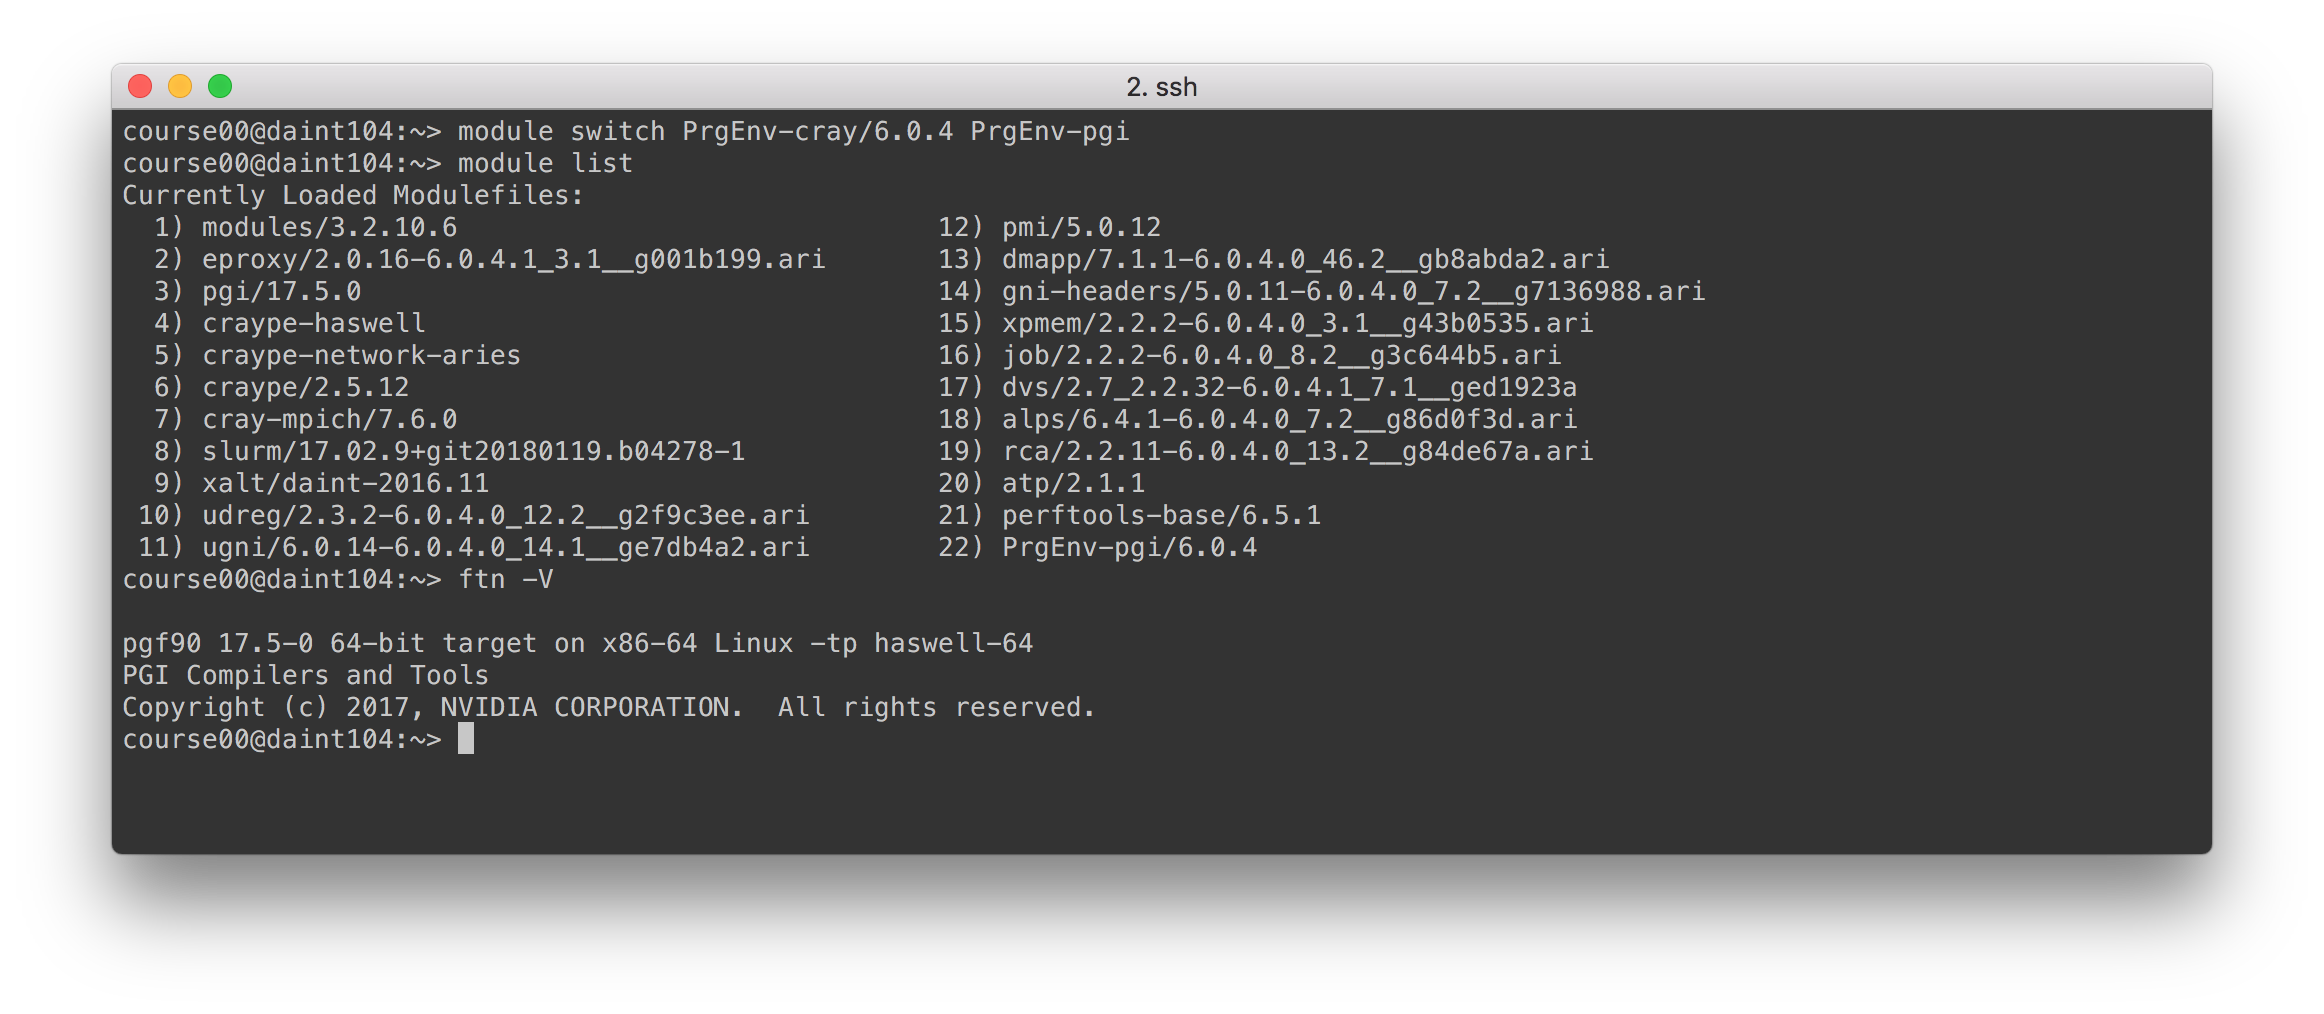
\includegraphics[width=\textwidth]{module_switch.png}
  }
\end{frame}

\begin{frame}{Managing programming environments}{Switching back to the Cray programming environment}
  {
    \centering
    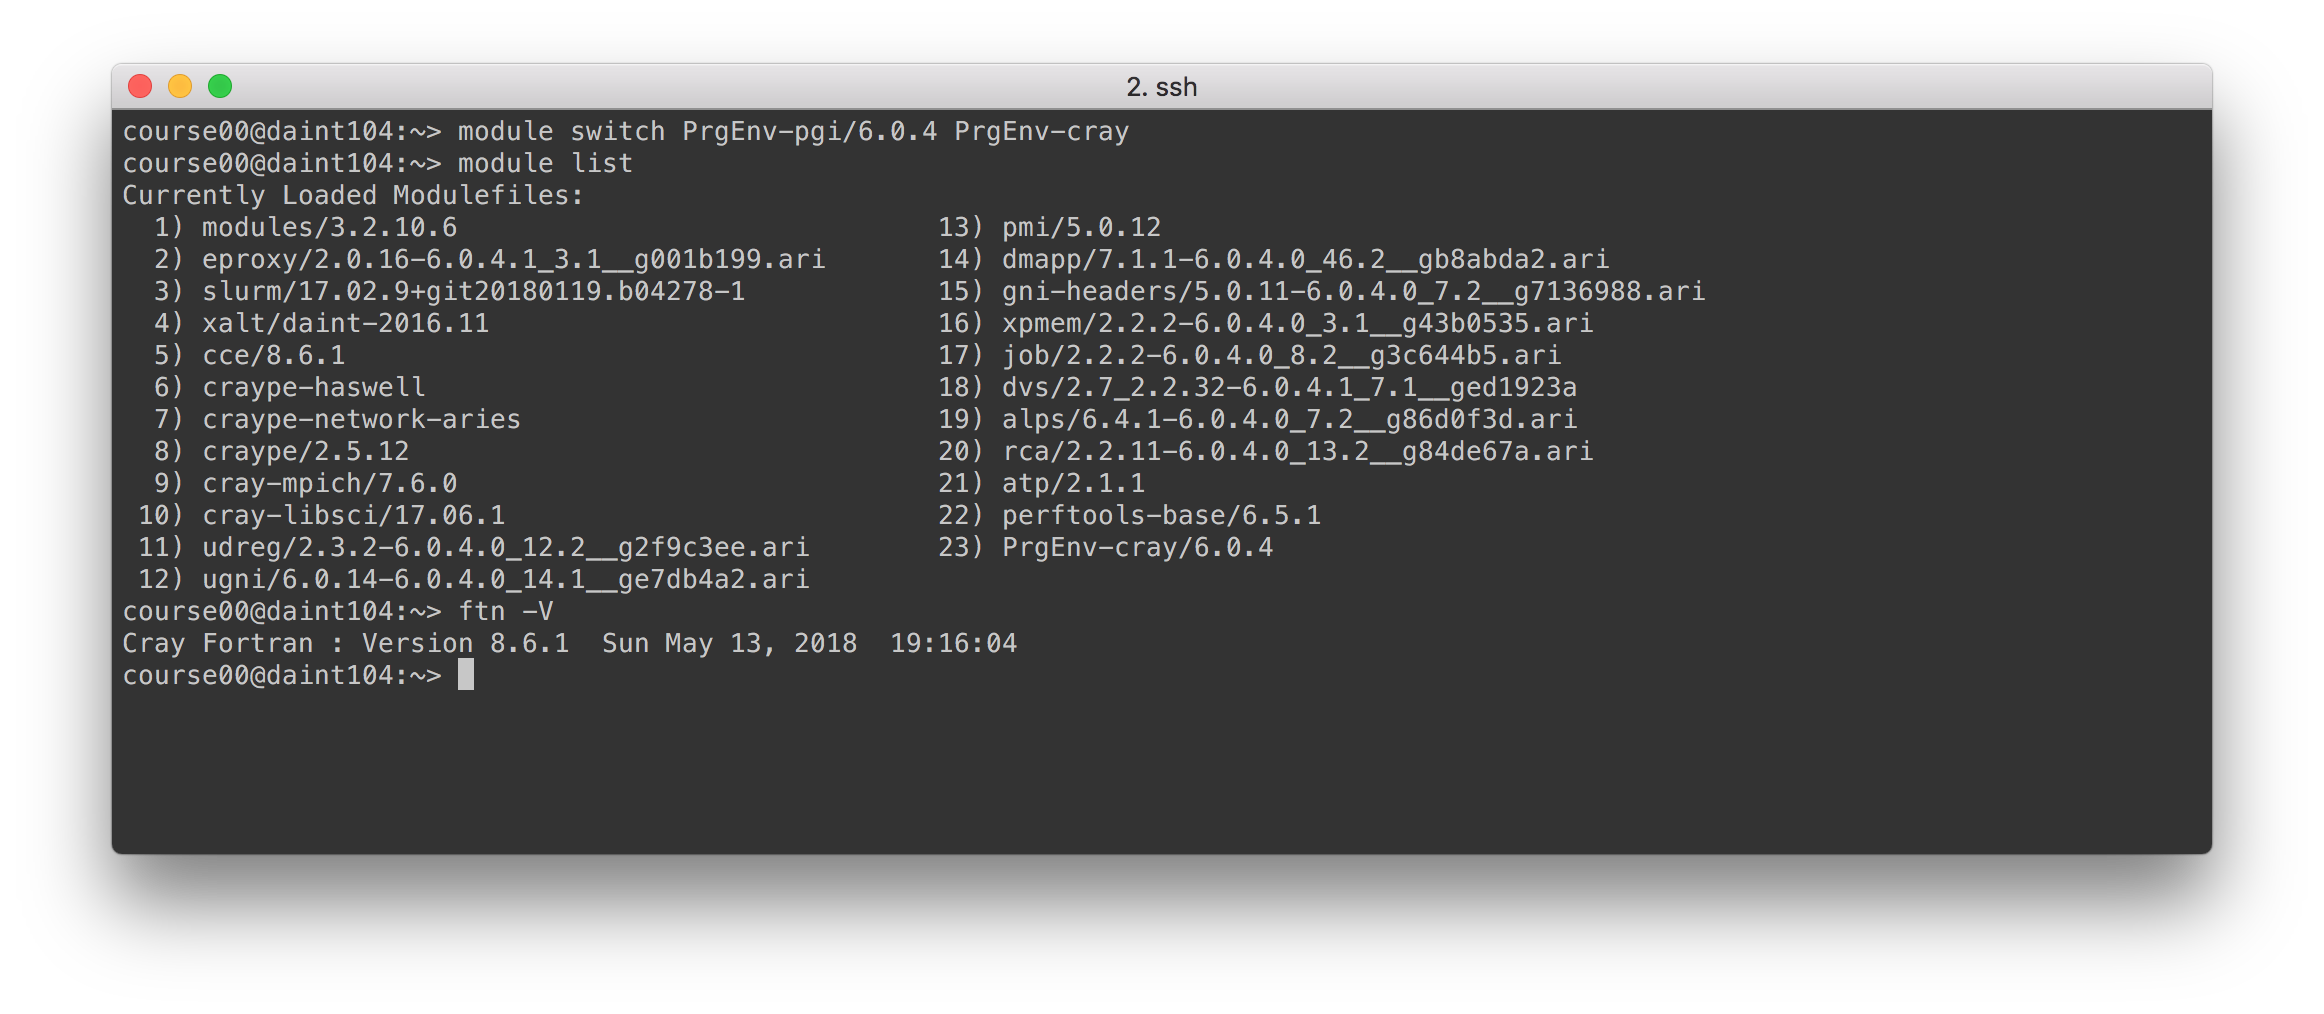
\includegraphics[width=\textwidth]{module_switch_cray.png}
  }
\end{frame}

\begin{frame}{Managing programming environments}{Loading and unloading modules}
  \begin{itemize}
  \item[--] \shinline{module load [MODULE_NAME]}
  \item[--] \shinline{module unload [MODULE_NAME]}
  \end{itemize}

  {
    \centering
    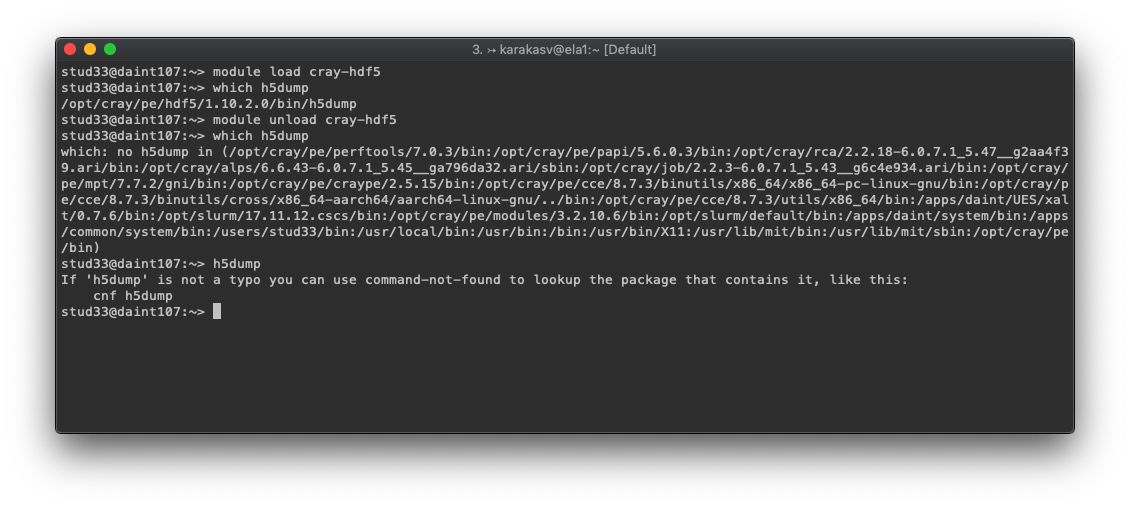
\includegraphics[width=\textwidth]{module_load_unload.png}
  }
\end{frame}


\begin{frame}{Managing programming environments}{Checking available modules}
  \begin{itemize}
  \item[--] The \texttt{daint-gpu} makes available the CSCS software stack built for the hybrid nodes of the system
  \end{itemize}
  {
    \centering
    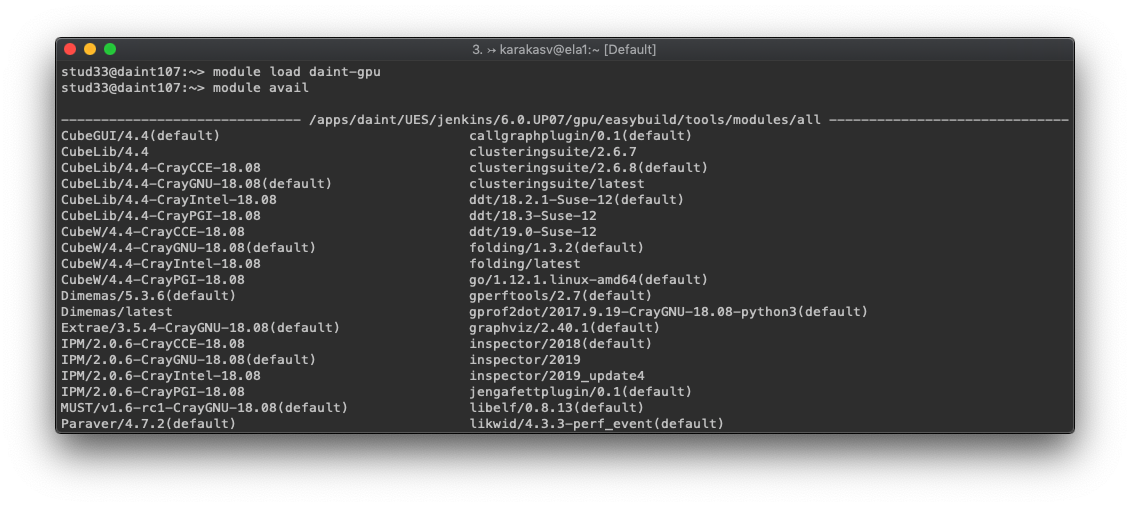
\includegraphics[width=\textwidth]{module_avail_all.png}
  }
\end{frame}

\begin{frame}{Managing programming environments}{Checking available modules}
  \begin{itemize}
  \item Check available versions of a software
  \end{itemize}
  {
    \centering
    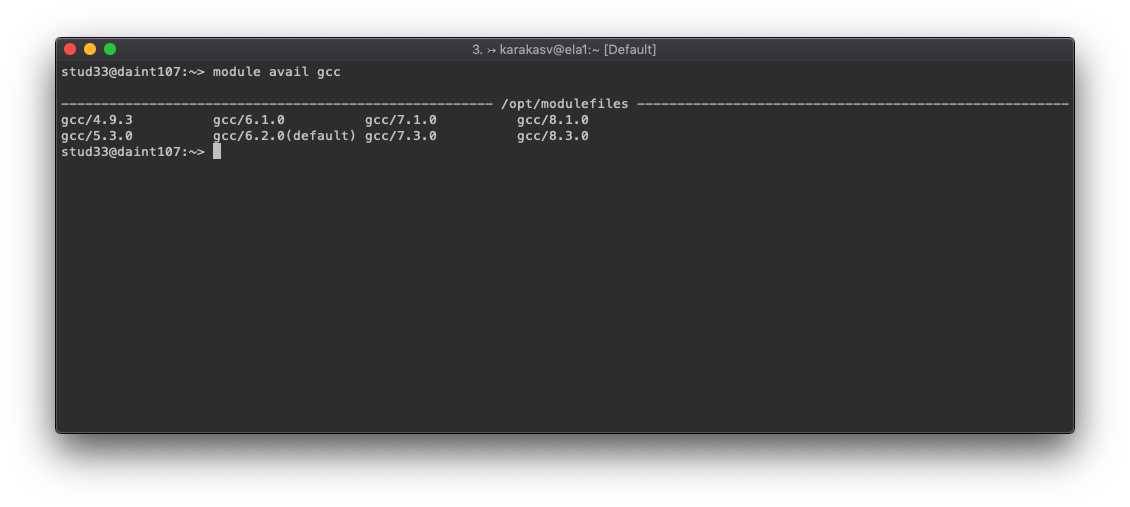
\includegraphics[width=\textwidth]{module_avail_gcc.png}
  }
\end{frame}

\begin{frame}{Managing programming environments}{Get information about a module}
  \begin{itemize}
  \item[--] Environment variables set, paths etc.
  \end{itemize}

  {
    \centering
    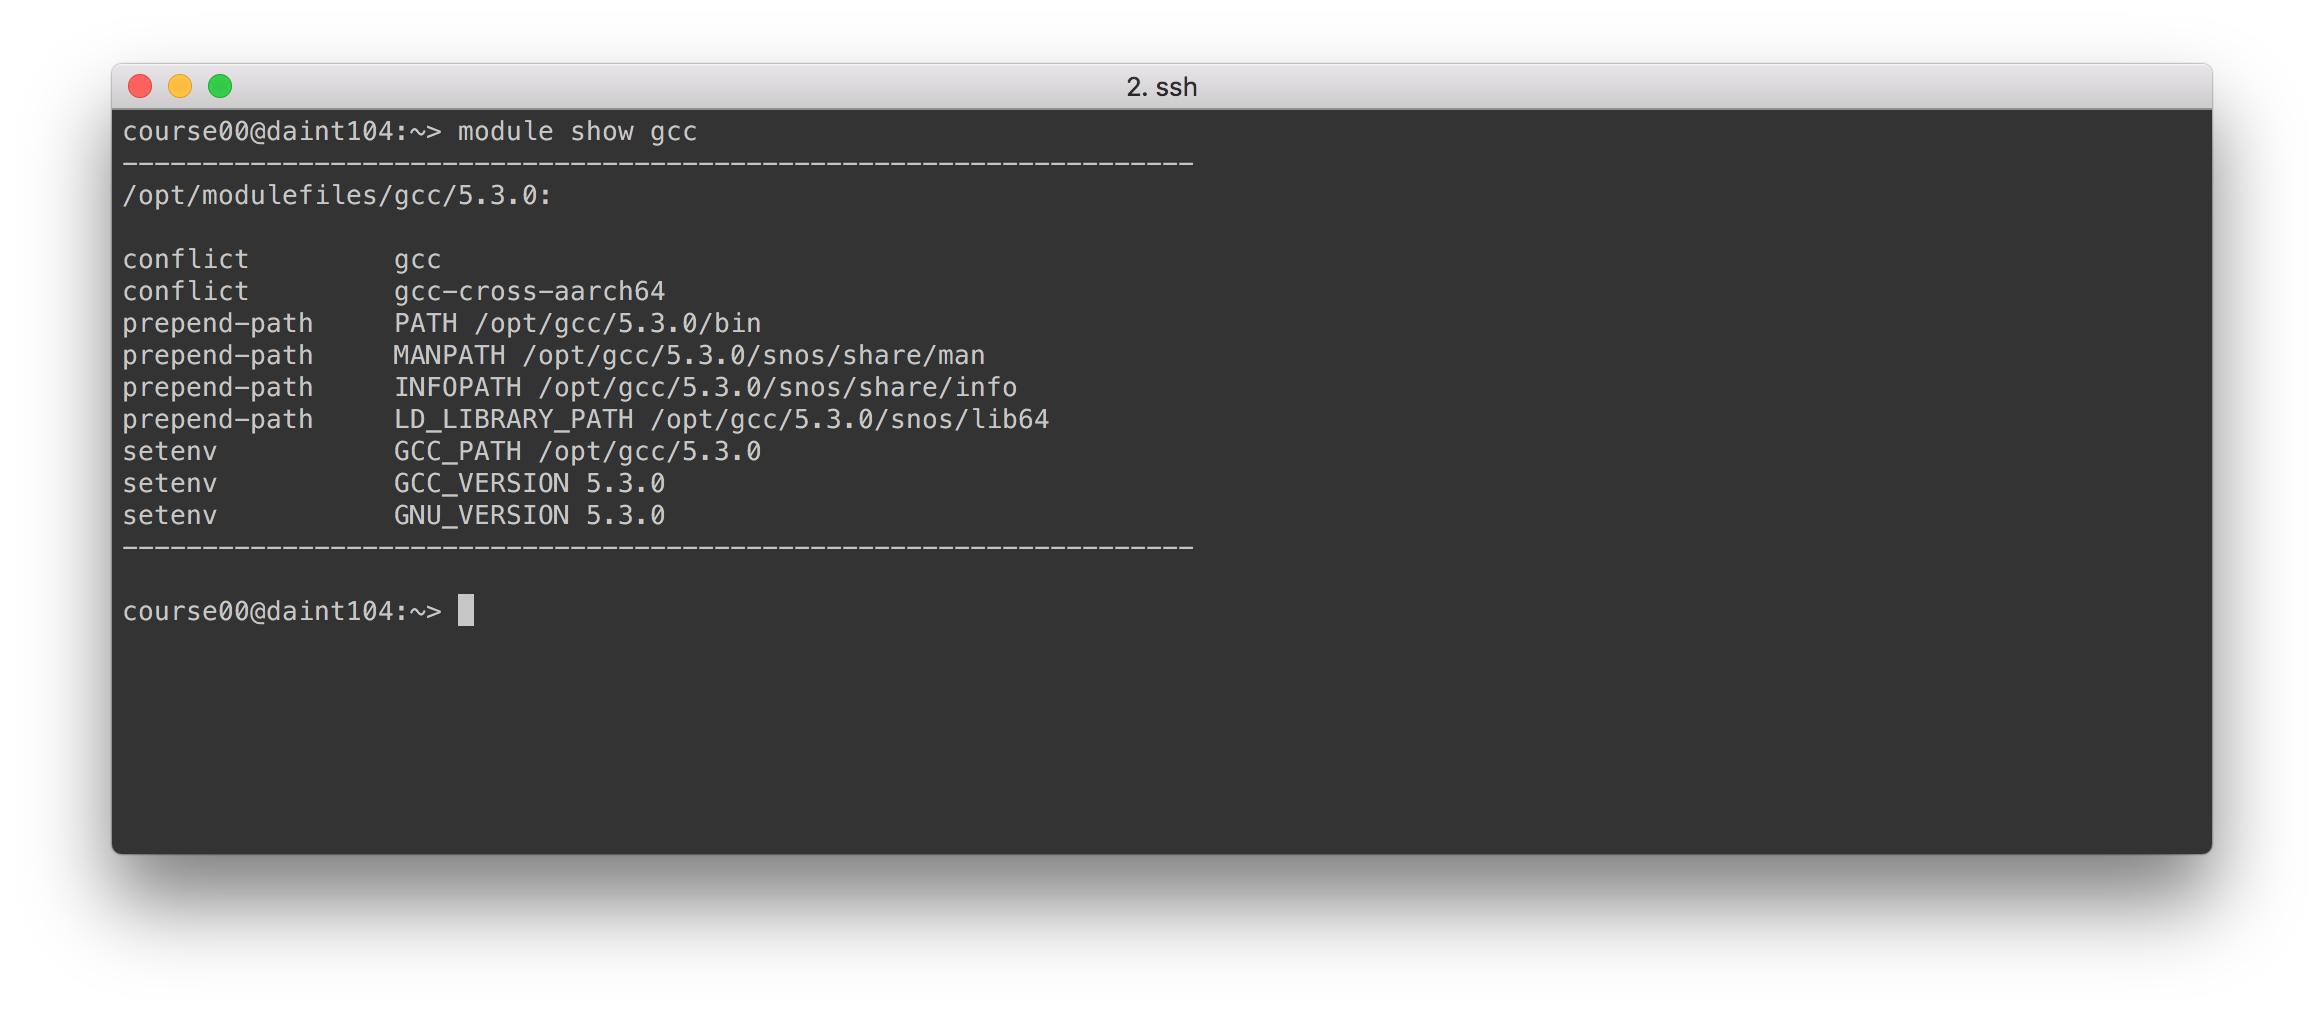
\includegraphics[width=\textwidth]{module_show_gcc.png}
  }
\end{frame}


\begin{frame}{Managing programming environments}{Get help for a module}
  {
    \centering
    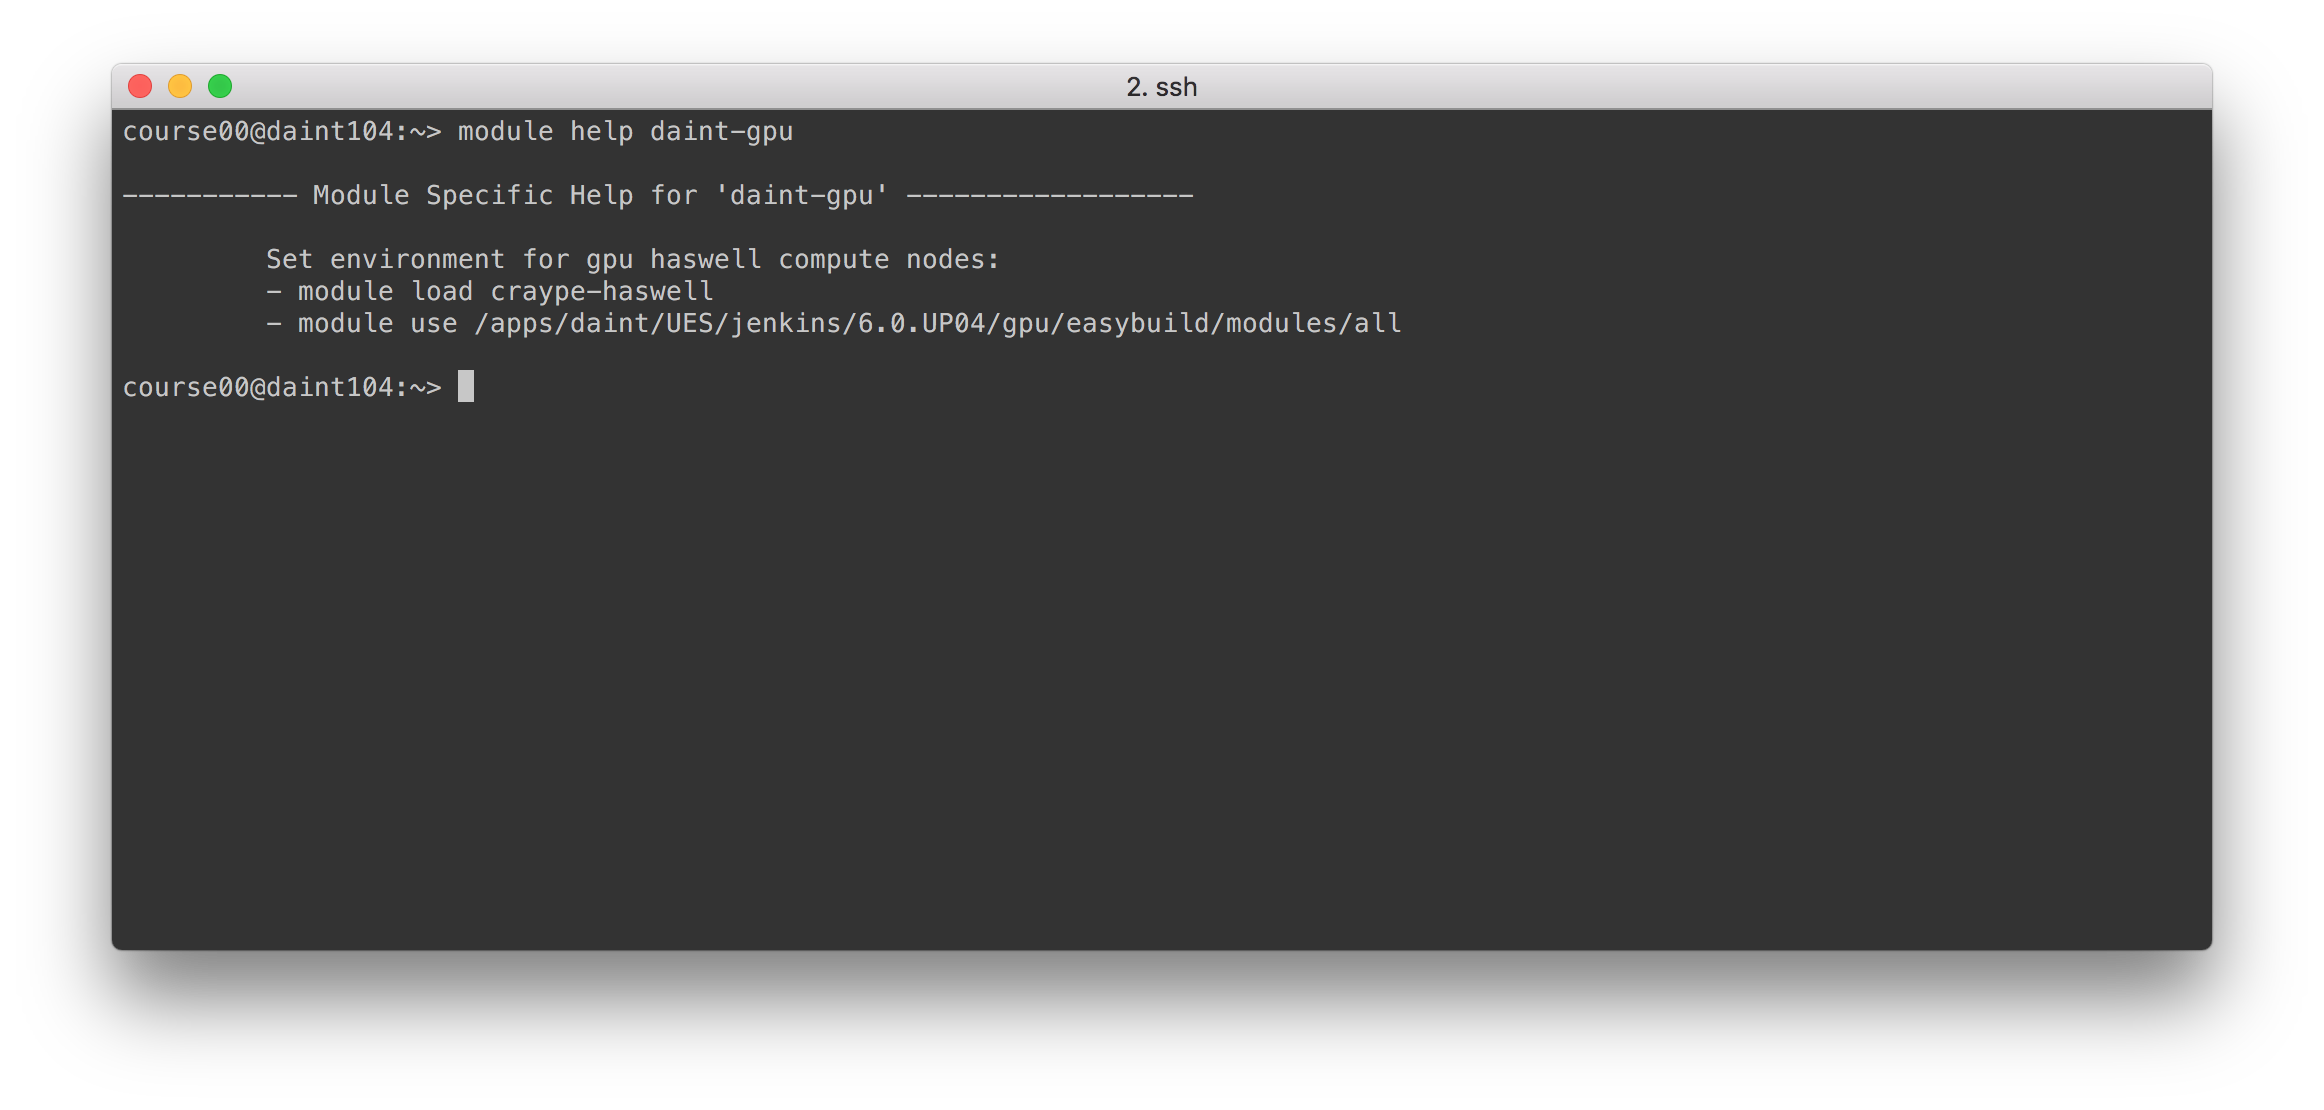
\includegraphics[width=\textwidth]{module_help_daint_gpu.png}
  }
\end{frame}

\begin{frame}{Running on Piz Daint}{The job scheduler}
  Piz Daint uses native SLURM for running jobs on the compute nodes.
  There are three ways of submitting a job:
  \vspace\baselineskip
  \begin{enumerate}
  \item Interactively from the login nodes using the \texttt{srun} command.
  \item By submitting a job script using the \texttt{sbatch} command.
  \item By pre-allocating resources using the \texttt{salloc} command.
  \end{enumerate}
\end{frame}

\begin{frame}[fragile]{Running on Piz Daint}{Using the \texttt{srun} command}
  Necessary and useful options:
  \begin{itemize}
  \item \texttt{-C gpu}: requests allocation on the hybrid (GPU) nodes (required)
  \item \texttt{--reservation=summer\_school}
    \begin{itemize}
    \item 64 nodes valid until Jul.\ 25 @ 13:00.
    \end{itemize}
  \item \texttt{-N 2}: number of compute nodes (default is 1)
  \item \texttt{-n 2}: number of MPI tasks (default is 1)
  \item \texttt{-t 5}: maximum duration of the job (default is 30min)
    \begin{itemize}
    \item Allows to get an allocation quicker
    \item Job will be killed if time limit is reached
    \item Maximum time slot for a job is 24h
    \end{itemize}
  \end{itemize}
  More on \url{https://user.cscs.ch/access/running}
\end{frame}

\begin{frame}[fragile]{Running on Piz Daint}{Using the \texttt{srun} command}
  {
    \centering
    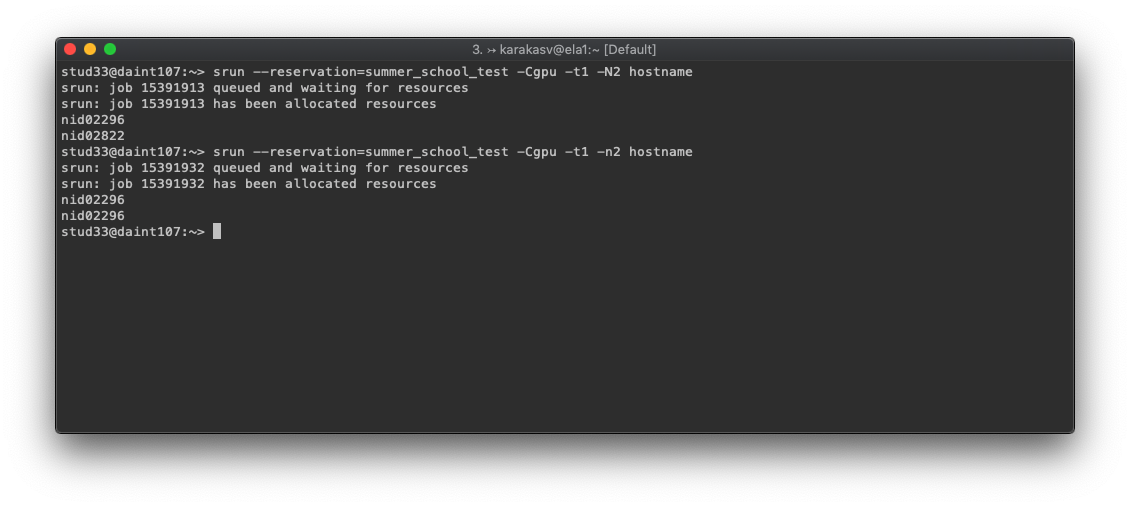
\includegraphics[width=\textwidth]{srun_hostname.png}
  }
\end{frame}

\begin{frame}[fragile]{Running on Piz Daint}{Using the \texttt{sbatch} command}
  {
    \centering
    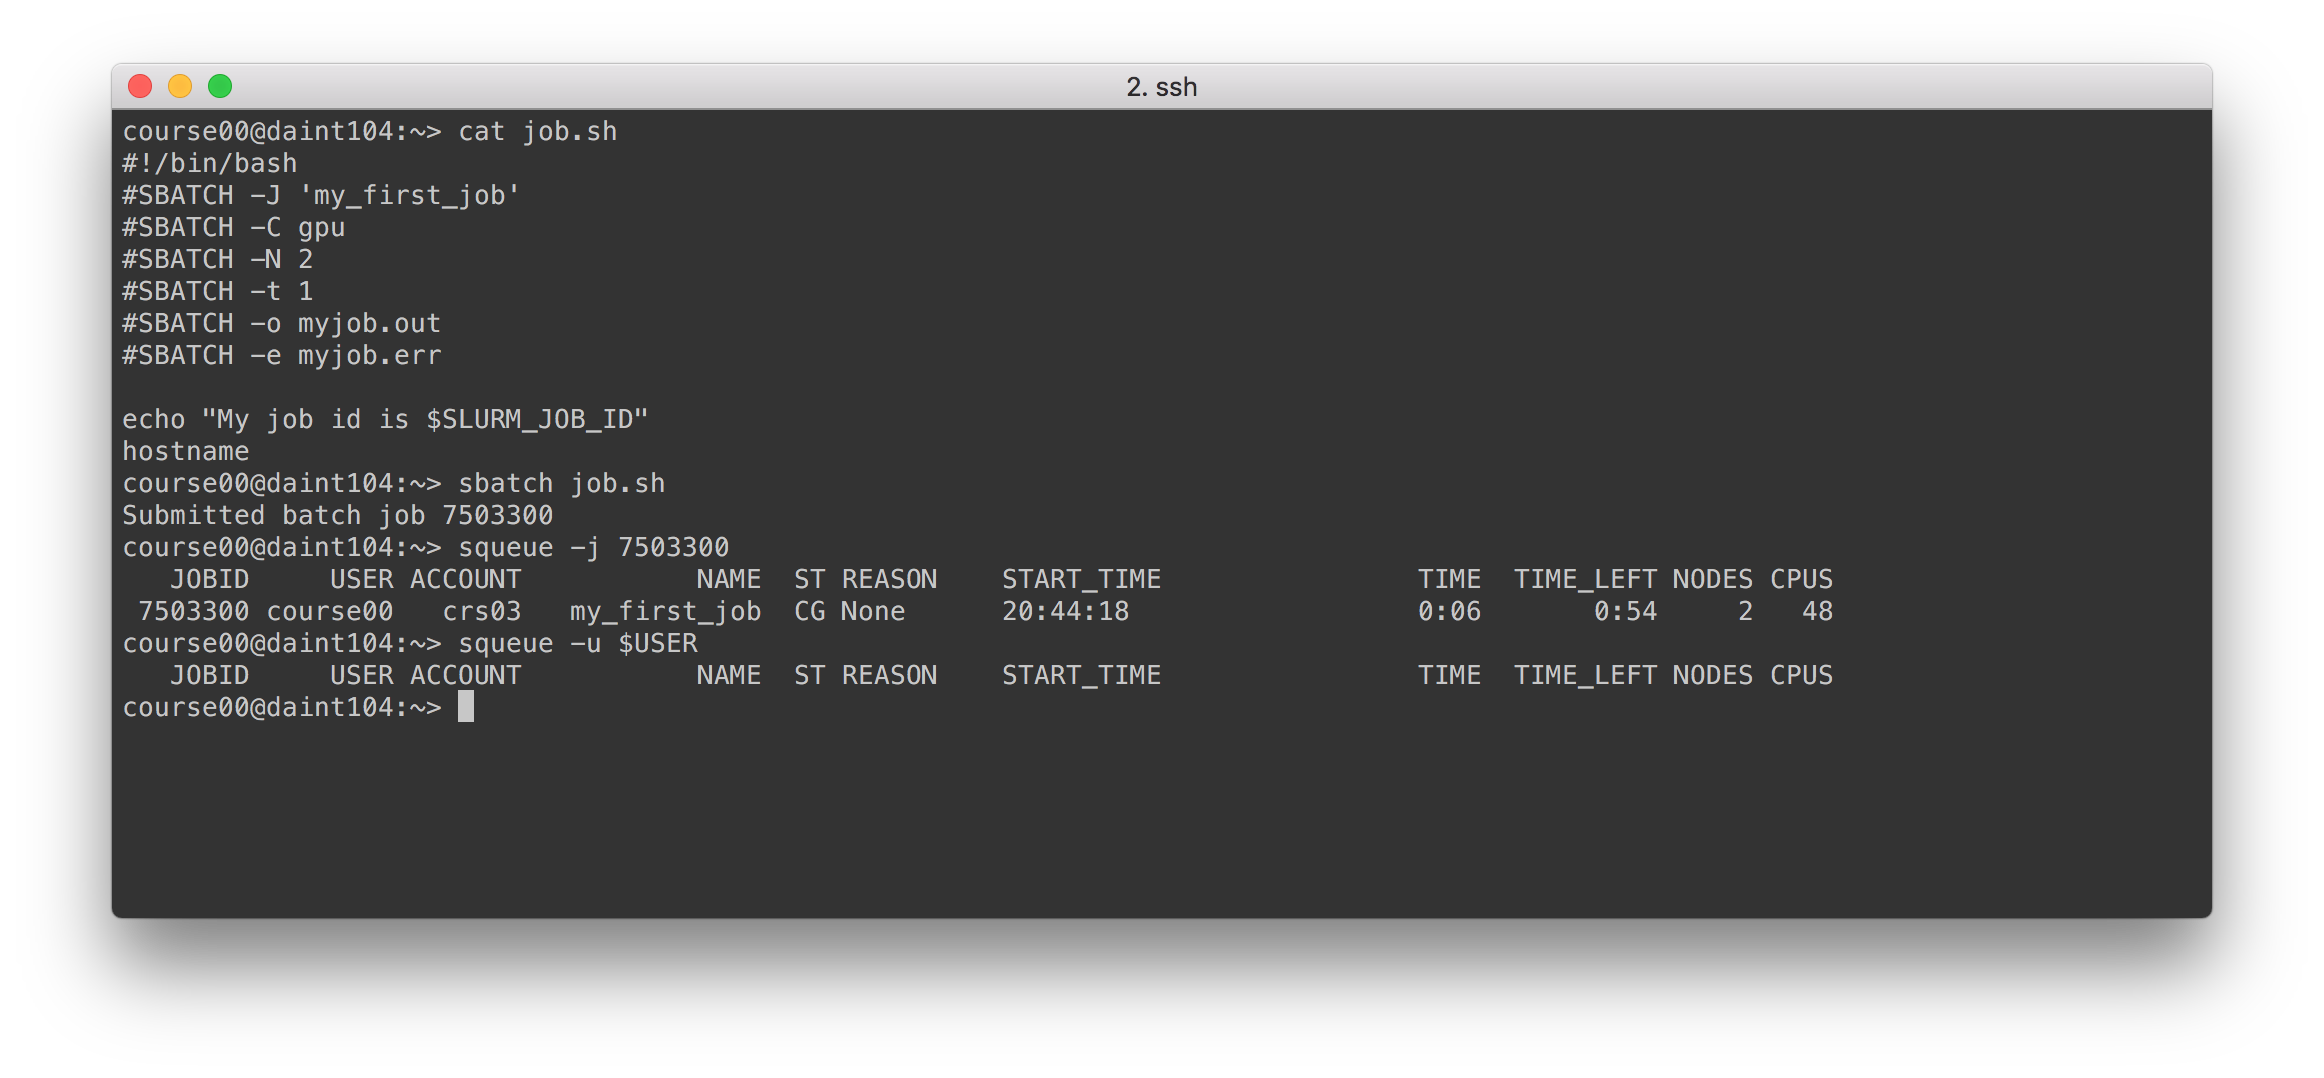
\includegraphics[width=\textwidth]{sbatch_hostname.png}
  }
\end{frame}


\begin{frame}[fragile]{Running on Piz Daint}{Using the \texttt{sbatch} command -- Examinining the output}
  {
    \centering
    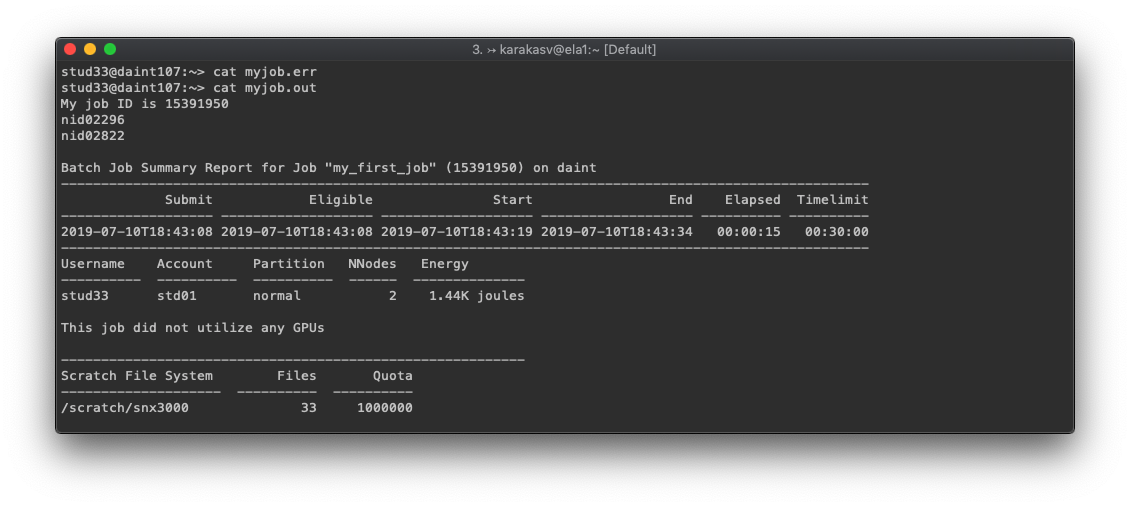
\includegraphics[width=\textwidth]{sbatch_hostname_output.png}
  }
\end{frame}

\begin{frame}[fragile]{Running on Piz Daint}{Using the \texttt{salloc} command}
  {
    \centering
    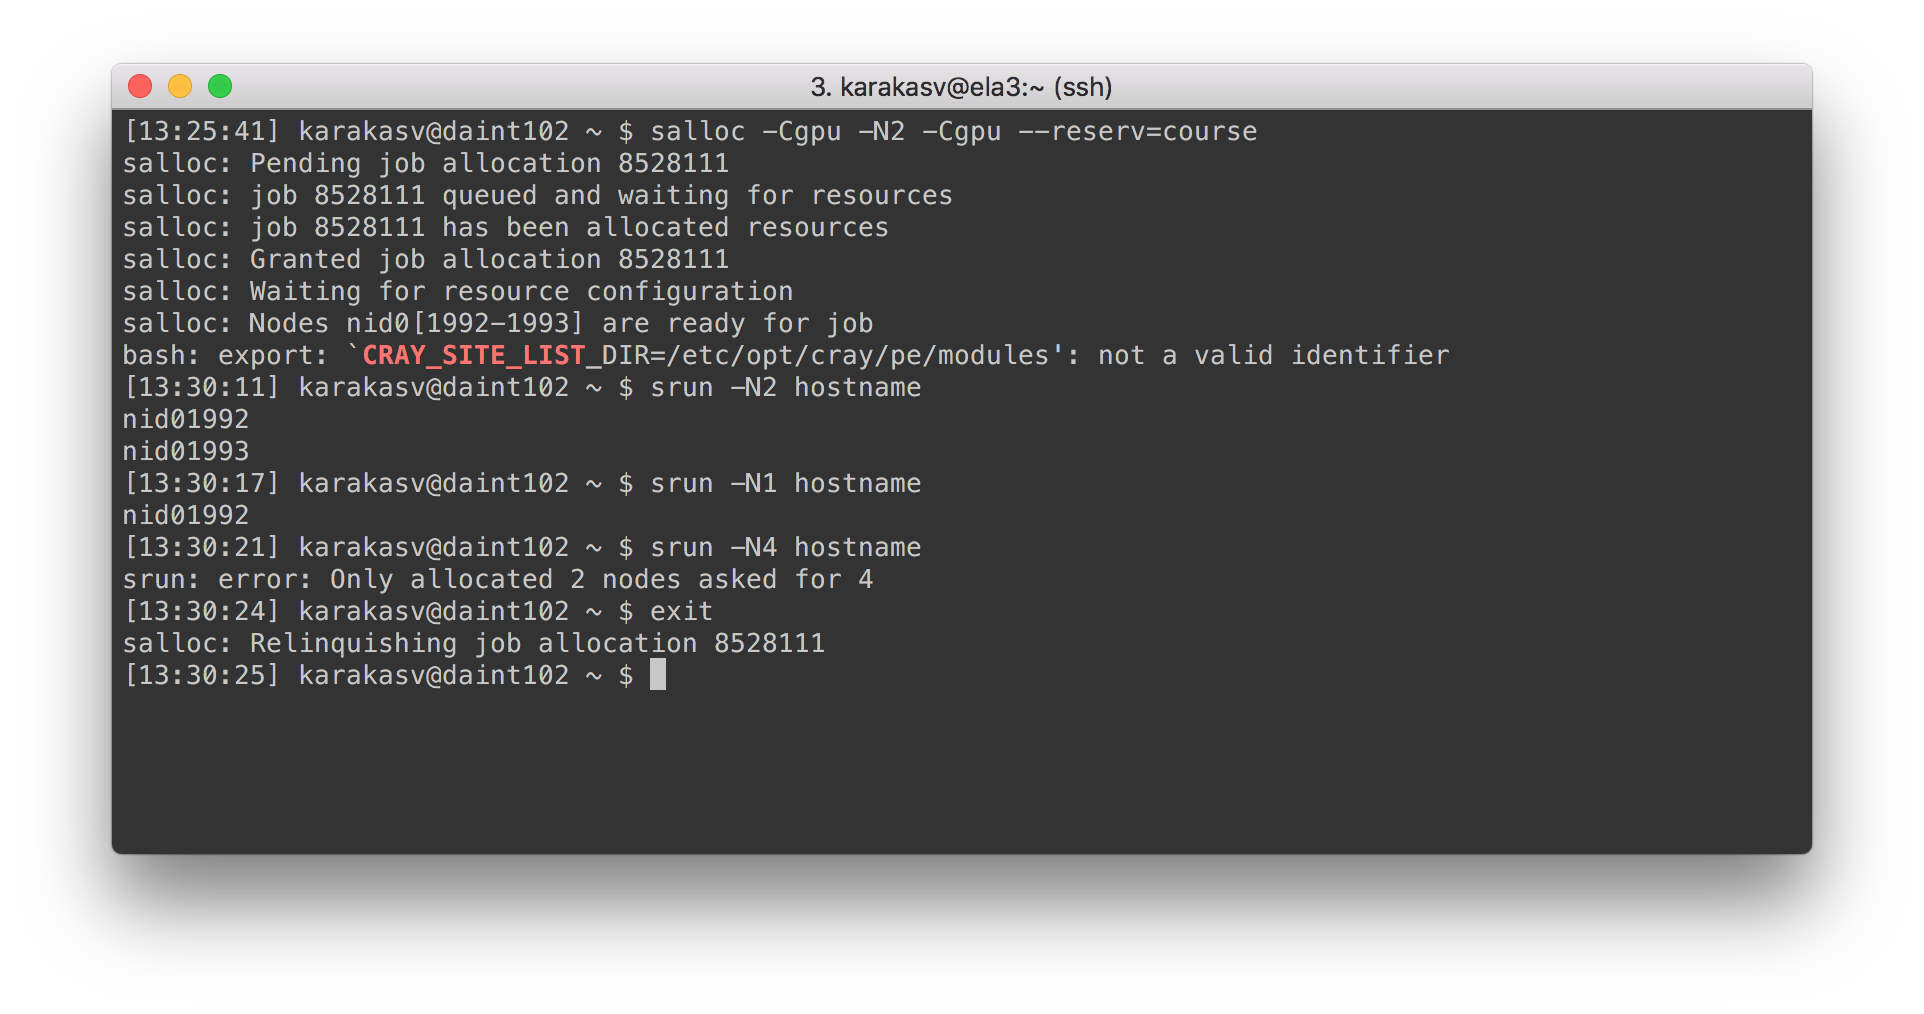
\includegraphics[width=\textwidth]{salloc_hostname.png}
  }
\end{frame}

\begin{frame}{Running on Piz Daint}{Other useful commands}
  \begin{itemize}
  \item \texttt{squeue [OPTIONS]}: Check the status of the system job queue
    \begin{itemize}
    \item Useful options: \texttt{-u [USERNAME]}, \texttt{-j [JOBID]}
    \end{itemize}
  \item \texttt{scancel [JOBID]}: Cancel a job
  \item \texttt{scontrol}: Detailed information about partitions, reservations,
    computing nodes etc.
  \end{itemize}
\end{frame}

\begin{frame}{Running on Piz Daint}{Other useful commands}
  {
    \centering
    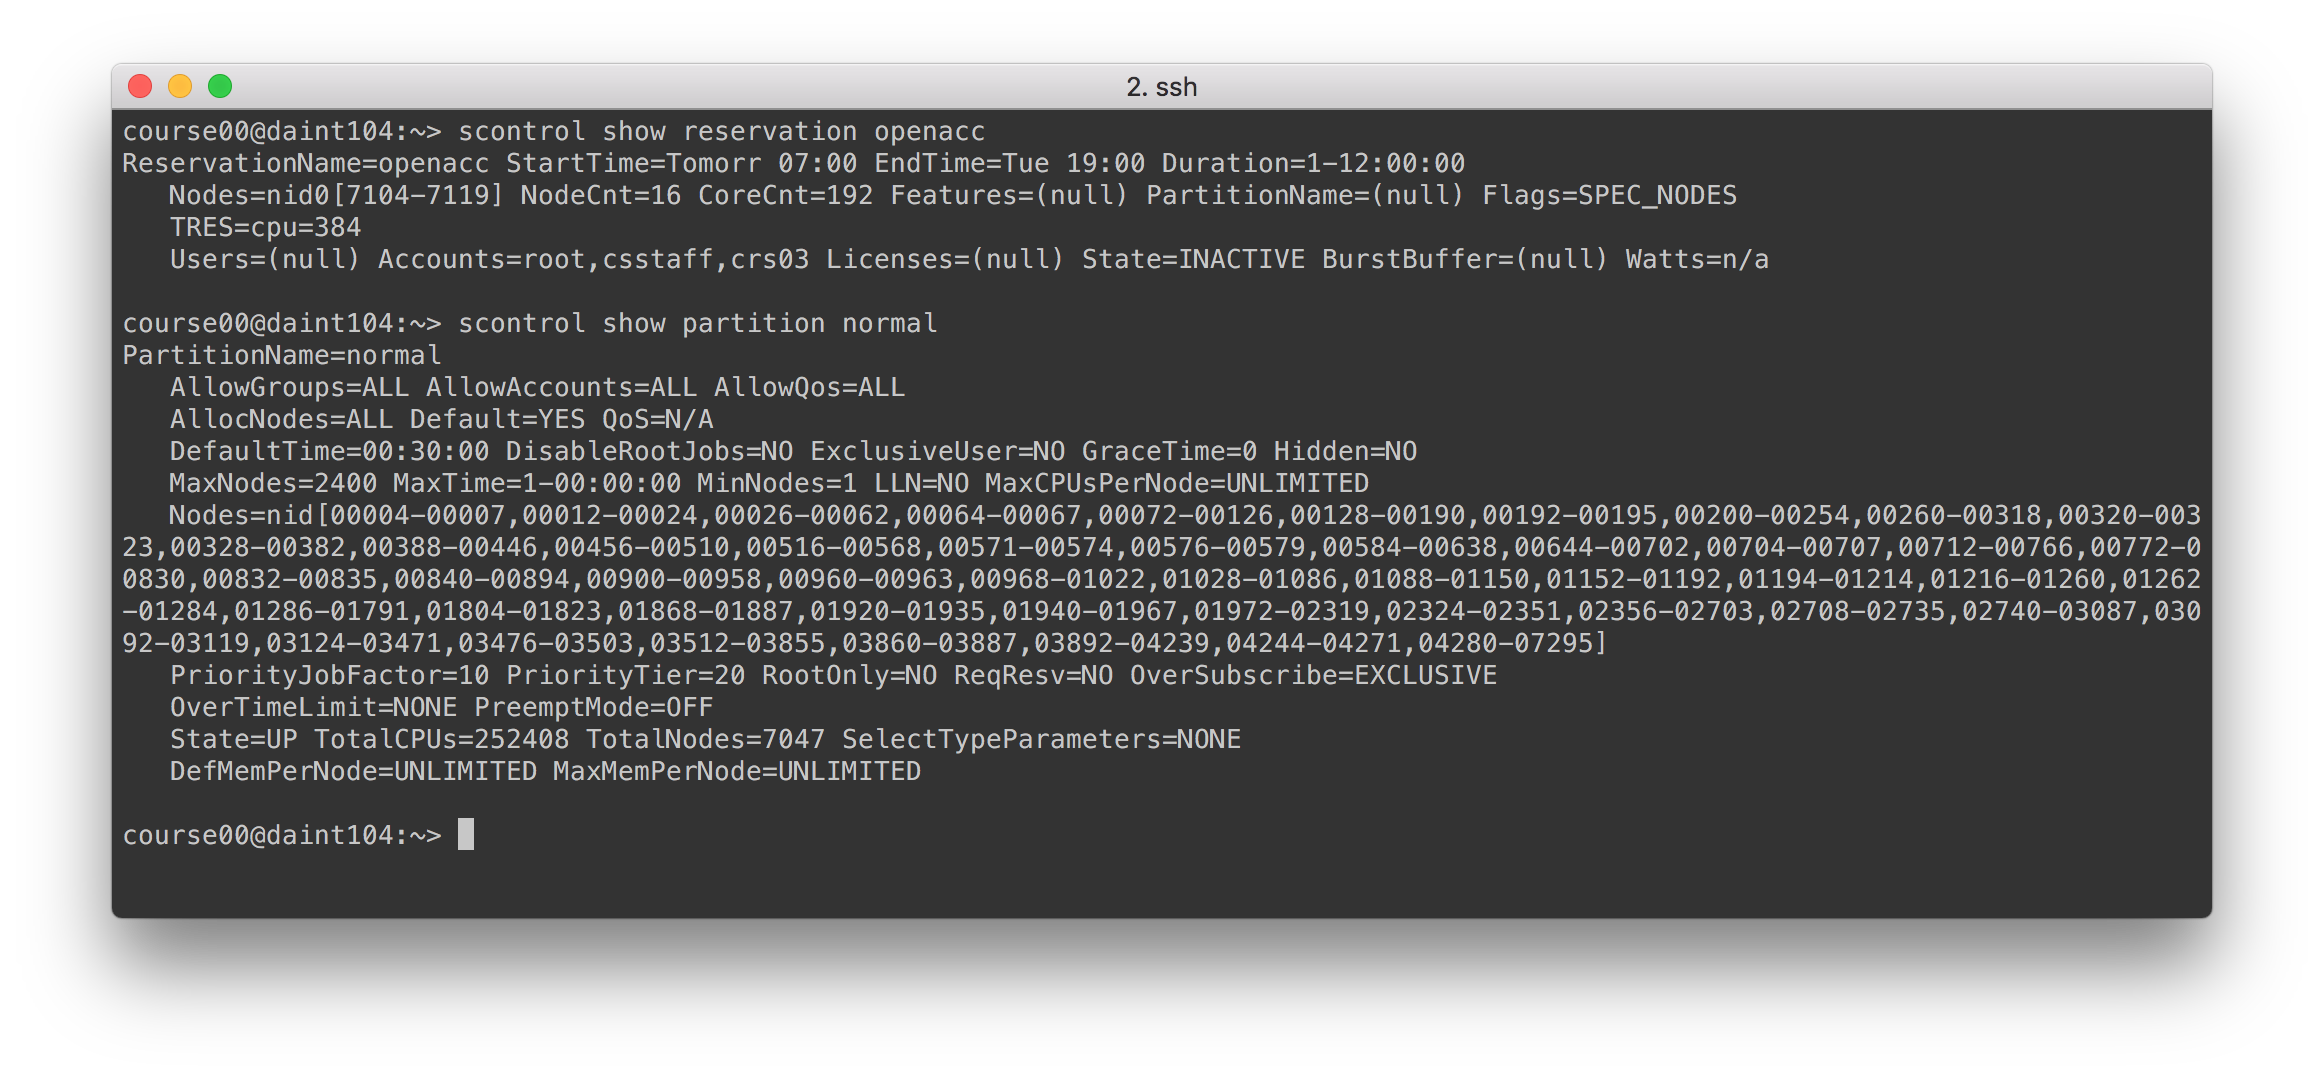
\includegraphics[width=\textwidth]{scontrol.png}
  }
\end{frame}

\begin{frame}{Editing files}
  \begin{itemize}
  \item \texttt{vim} or \texttt{gvim} (X version)
  \item \texttt{emacs -nw} or just \texttt{emacs} (X version)
  \item \texttt{gedit} (X only)
  \end{itemize}
\end{frame}

\begin{frame}{Moving data to/from CSCS}
  \begin{itemize}
  \item \texttt{scp}: Remote copy over SSH
    \begin{itemize}
    \item Getting a file: \shinline{scp studXX@ela.cscs.ch:remotefile localfile}
    \item Getting a directory: \shinline{scp -r studXX@ela.cscs.ch:remotedir localdir}
    \item Sending a file: \shinline{scp localfile studXX@ela.cscs.ch:remotefile}
    \item Sending a directory: \shinline{scp localdir studXX@ela.cscs.ch:remotedir}
    \end{itemize}
  \item \texttt{rsync}: Synchronize files remotely over SSH
    \begin{itemize}
    \item \shinline{rsync -avz studXX@ela.cscs.ch:remotedir/ localdir/}
    \item \shinline{rsync -avz localdir/ studXX@ela.cscs.ch:remotedir/}
    \item Pay attention to the slashes! \shinline{rsync} \emph{behaves differently
      with or without slashes.}
    \end{itemize}
  \end{itemize}
\end{frame}


\end{document}
